\documentclass[12pt]{article}
\usepackage{listings}
\usepackage{color}
\usepackage{float}
\usepackage{graphicx}

\definecolor{mygreen}{rgb}{0,0.6,0}
\definecolor{mygray}{rgb}{0.5,0.5,0.5}
\definecolor{mymauve}{rgb}{0.58,0,0.82}

\lstset{ %
	xleftmargin=2em,
	backgroundcolor=\color{white},   % choose the background color; you must add \usepackage{color} or \usepackage{xcolor}
	basicstyle=\small,%\footnotesize,        % the size of the fonts that are used for the code
	breakatwhitespace=false,         % sets if automatic breaks should only happen at whitespace
	breaklines=true,                 % sets automatic line breaking
	captionpos=t,                    % sets the caption-position to bottom
	commentstyle=\color{mygreen},    % comment style
	deletekeywords={...},            % if you want to delete keywords from the given language
	escapeinside={\%*}{*)},          % if you want to add LaTeX within your code
	extendedchars=true,              % lets you use non-ASCII characters; for 8-bits encodings only, does not work with UTF-8
	%	frame=single,                    % adds a frame around the code
	keepspaces=true,                 % keeps spaces in text, useful for keeping indentation of code (possibly needs columns=flexible)
	keywordstyle=\color{blue},       % keyword style
	language=VHDL, % the language of the code
	morekeywords={*,...},            % if you want to add more keywords to the set
	numbers=left,                    % where to put the line-numbers; possible values are (none, left, right)
	numbersep=5pt,                   % how far the line-numbers are from the code
	numberstyle=\small\color{mygray}, % the style that is used for the line-numbers
	rulecolor=\color{black},         % if not set, the frame-color may be changed on line-breaks within not-black text (e.g. comments (green here))
	showspaces=false,                % show spaces everywhere adding particular underscores; it overrides 'showstringspaces'
	showstringspaces=false,          % underline spaces within strings only
	showtabs=false,                  % show tabs within strings adding particular underscores
	stepnumber=1,                    % step between two line-numbers. If it's 1, each line will be numbered
	stringstyle=\color{mymauve},     % string literal style
	tabsize=2                  % sets default tabsize to 2 spac                  % show the filename of files included with \lstinputlisting; also try caption instead of title
}
%opening
\title{\textbf{Project 3: Designing a 32-bit CPU}}
\author{\textbf{Adam Sumner} - A20283081, \textbf{Contribution} - 25\% \\
		\textbf{Bobby Unverzagt} - A2028923, \textbf{Contribution} - 25\% \\
		\textbf{Emilie Woog} - A20265269, \textbf{Contribution} - 25\% \\
		\textbf{Nash Kaminski} - A20283999, \textbf{Contribution} - 25\% \\ ~\\ ECE 485}
\date{December 5\textsuperscript{th}, 2015}

\begin{document}

\maketitle

\section{Introduction}
This goal of this project is to design a stripped down version of the MIPS processor. The processor will be a 32-bit version of the processor discussed in class and the text book, however, its instruction set will be a small subset of the MIPS processor's full capability. 

\subsection{Background Information}
\subsubsection{MIPS}
MIPS is a reduced instruction set computer (RISC) instruction set architecture (ISA). It defines three types of instruction types: R (register), I (Immediate), and J (Jump). For the implementation that this project is focused on, only R and I instructions will be executed. R type instructions are the most common form of instructions. The format for an r-type instruction is:

\begin{center}

\resizebox{\textwidth}{!}{\begin{tabular}{|c|c|c|c|c|c|}
	\hline
	\texttt{Bits[31:26]} & \texttt{Bits[25:21]} & \texttt{Bits[20:16]} & \texttt{Bits[15:11]} & \texttt{Bits[10:6]} & \texttt{Bits[5:0]} \\ \hline
	opcode & Rs & Rt & Rd & shamt & funct \\ \hline
	
\end{tabular}}
\end{center}

\noindent For this instruction, the opcode field is always $000000_2$, while the function code \texttt{funct} is used to determine which instruction is to be carried out. Rs and Rt are the two registers in which the operation reads and Rd is the destination of the result. Some instructions require a shift amount (\texttt{shamt}), so it is specified explicitly.
\\

\noindent The I type instruction involves an immediate value, so the instruction format must accommodate this. The format of this type of instruction is: \\
\begin{center}

\begin{tabular}{|c|c|c|c|}
	\hline
	\texttt{Bits[31:26]} & \texttt{Bits[25:21]} & \texttt{Bits[20:16]} & \texttt{Bits[15:0]} \\ \hline
	opcode & Rs & Rt & immediate \\ \hline
\end{tabular}

\end{center}

\noindent For this instruction, the op code field is used to define the specific instruction, Rs is the register in which the operation acts on along with the immediate value as the other operand. Rt is the destination register in which the result is stored.

\subsubsection{Datapath and Control}
A datapath is a collection of functional units that perform data processing operations. It includes units such as a program counter, a register file, instruction memory, an ALU, data memory, and a control unit. Figure \ref{fig:textbook-datapth} shows a high level overview of a simple datapath with control.
\begin{figure}[H]
\centering
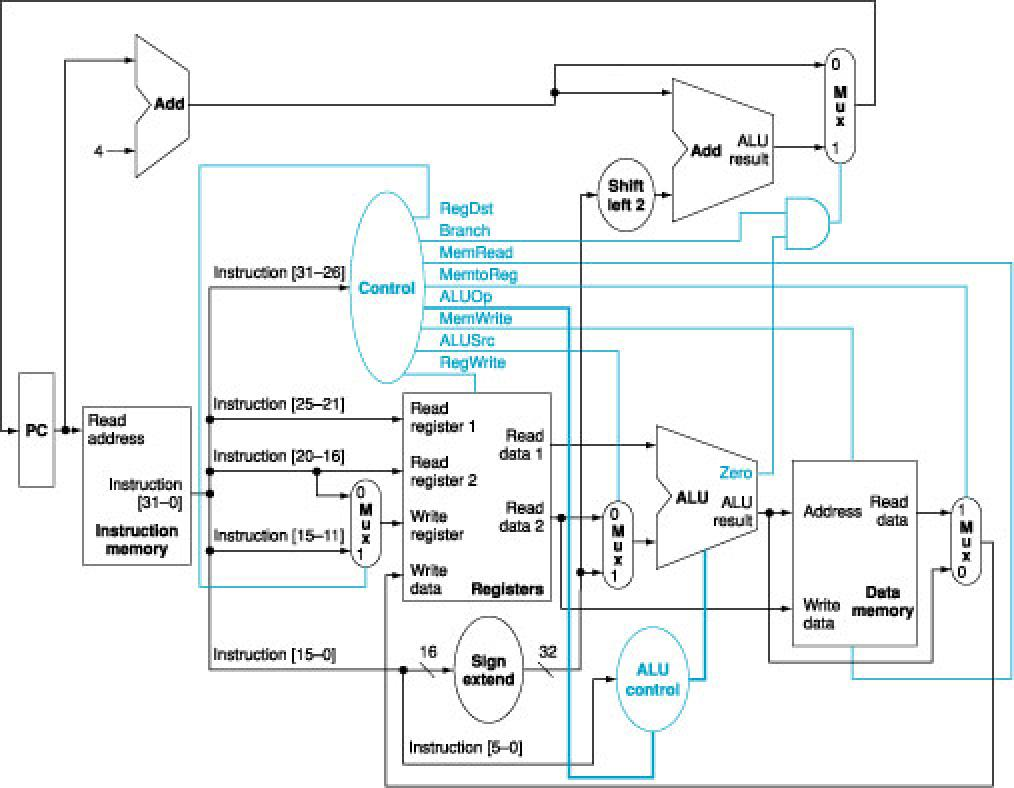
\includegraphics[width=\linewidth]{textbook-datapth}
\caption{Datapath Overview}
\label{fig:textbook-datapth}
\end{figure}

\newpage
\section{Design}
\subsection{Instruction Set}
Table \ref{tab:operations} shows the instructions that were chosen to be implemented in the CPU with the respective OpCode and Function Field for each instruction.
\begin{table}[H]
	\centering
	\begin{tabular}{|c|c|c|l|}
		\hline
		\texttt{OpCode[31:26]} & \texttt{Function Field [5:0]} & Instruction & 
		Example Operation \\ 
		\hline
		$100011_2$ & \texttt{--} & \texttt{lw} & \texttt{lw \$t3, 200(\$s2)}  \\
		\hline
		$101011_2$ & \texttt{--} & \texttt{sw} & \texttt{sw \$t4, 100(\$t3)} \\
		\hline
		$000000_2$ & $100000_2$ & \texttt{add} & \texttt{add \$s3, \$t2, \$s2} \\
		\hline
		$000000_2$ & $110000_2$ & \texttt{sub}& \texttt{sub \$s3, \$t2, \$s2}\\
		\hline
		$000100_2$ & \texttt{--} & \texttt{beq}&\texttt{beq \$s5, \$s2, 500}\\
		\hline
		$000000_2$ & $000001_2$ & \texttt{nand}& \texttt{nand \$s5, \$s1, \$s2} \\
		\hline
		$000010_2$ & \texttt{--} & \texttt{andi}& \texttt{andi \$s6, \$s2, 0x00FF} \\
		\hline
		$000000_2$ & $000010_2$ & \texttt{or}& \texttt{or \$s8, \$s1, \$s2} \\
		\hline
		$000011_2$ & \texttt{--} & \texttt{ori}& \texttt{ori \$s7, \$s1, 0x00FF} \\
		\hline		
	\end{tabular}
	\caption{CPU Instruction Set}
	\label{tab:operations}
\end{table}

\noindent Because it was only required to implement 9 instructions and the MIPS instruction set format requires 6 bits for op code and function field, it was an easy decision to choose these values for the implemented instructions. For all R-type instructions, the functions fields were chosen to be vastly different from one another to make debugging easier for the team. Likewise, the same approach was taken for the op code decisions for the I-type instructions.
\subsection{Memory}\label{sec:memory}
For this project, it seemed unnecessary to implement memory of 4GB ($2^{32}$). It was chosen to use an array of 256 words instead. If need be, this memory size could be upgraded easily, so this choice does not hinder performance on the actual design of the CPU.
\subsection{Datapath}
Because of the simplicity of this design, the implemented datapath did not need to be modified by much from Figure \ref{fig:textbook-datapth}. Therefore, the design of a single cycle datapath from the textbook acted as the skeletal structure of the final implementation. Because an ALU and Register file were previously implemented in earlier projects, it was necessary to extend their functionality to be able to handle 32-bit words. Once this was complete, this left the data memory entity to be completed so that it could be included in the processor entity. As mentioned earlier in Section \ref{sec:memory}, this entity contains an array of 256 words, and allows for reading and writing.
\\

\noindent The processor entity combines all of the components into the desired datapath. It synchronizes the clock of the instruction memory, data memory, and register file so that the entire system is in sync with an external clock signal. The program counter is updated during the rising edge of the clock, and all writes happen on the falling edge. The processor relies on the control unit to carry out the instruction read from memory.
Figure \ref{fig:datapth} shows the overview block diagram of the implemented datapath for the CPU.
\begin{figure}[H]
\centering
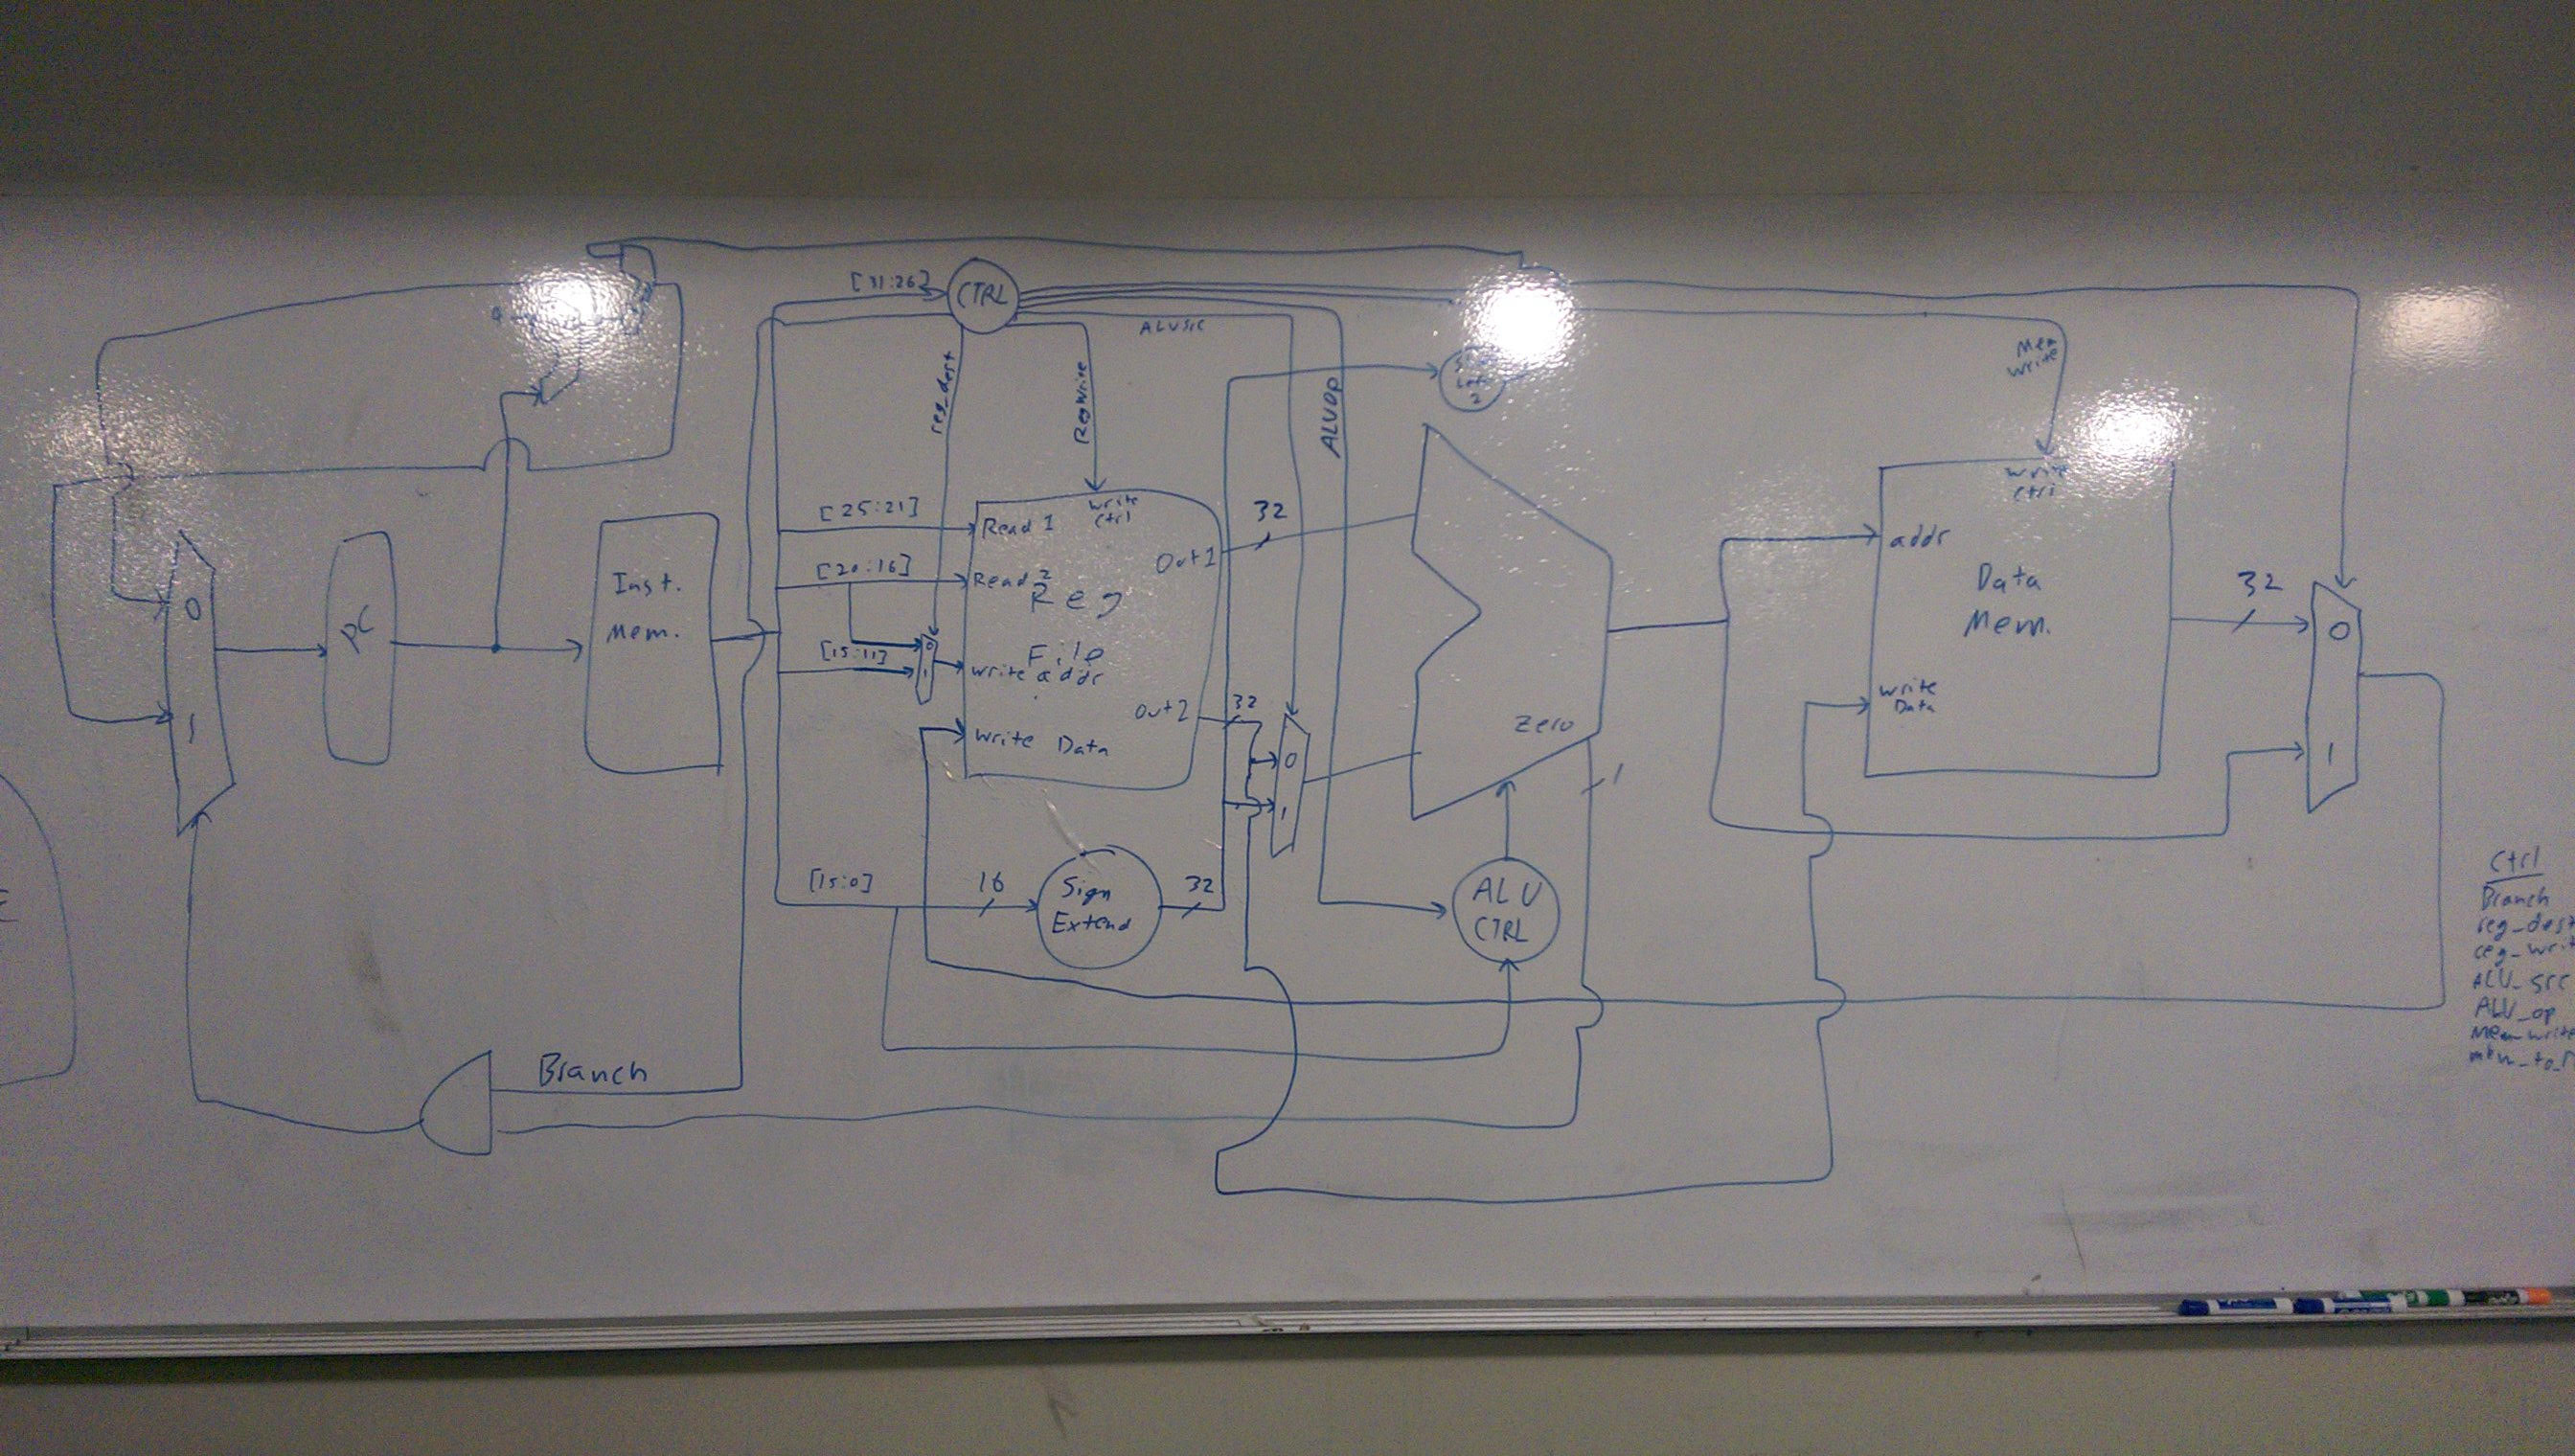
\includegraphics[width=\linewidth]{datapth}
\caption{Implemented Data Path Overview}
\label{fig:datapth}
\end{figure}

\subsection{Control}
The control lines can also be seen in Figure \ref{fig:datapth}. It is a simple design of several signals acting as the \texttt{sel} line of a series of multiplexers. Based on the op codes and function field read from the instruction memory, the signals are asserted accordingly to relay the correct signals into the Register File, ALU, and Data memory. This unit is what determines which units will read/write, and what operations the ALU should perform.
\section{Analysis}
While this processor was optimized to be able to fully accomplish the tasks specified in the business requirements document, it could still be improved. In its current stage, it can be considered a bare bones prototype. To transform the current design into a processor on par with the current industry standard, a complete instruction set would have to be implemented. Furthermore, pipelining is a necessity to add. Any processor that doesn't implement pipelining is not making efficient use of its own components. After pipelining is implemented, hazard controls would need to coexist. This would allow for cool features of the processor to exist such as forwarding, making it a truly efficient piece of hardware.
\section{Simulation Results}
Once the processor was completely designed, it was necessary to write some test bench code. To test each instruction, data had to first be written to memory, along with the program being loaded onto the CPU. Due to the amount of signals involved in the CPU, not all will be shown in the simulation. The clock, contents of the registers, data memory, and program counter will only be shown. Data Memory addresses 0x00000001 $\to$ 0x00000005 were initialized with starting data. For simplicity, register numbers 1 $\to$ 8 are s registers. This is not the convention in a usual MIPS implemented processor, however, for testing the instructions, this assignment is arbitrary. Please refer to the Test Bench Code in the Appendix for a detailed view of the testing procedure. The execution of the program begins at 38ns. The tested instructions are:

\begin{enumerate}
	\item \texttt{lw \$s1, 1(\$zero)}
	\item \texttt{sw \$s1, 6(\$zero)}
	\item \texttt{lw \$s2, 2(\$zero)}
	\item \texttt{add \$s3, \$s1, \$s2}
	\item \texttt{sub \$s4, \$s2, \$s1}
	\item \texttt{beq \$s1, \$s2, 100}
	\item \texttt{lw \$2, 4(\$zero)}
	\item \texttt{nand \$s5, \$s1, \$s2}
	\item \texttt{andi \$s6, \$s2, 0x00FF}
	\item \texttt{ori \$s7, \$s1, 0x00FF}
	\item \texttt{or \$s8, \$s1, \$s2}
	\item \texttt{beq \$s1, \$s1, -0x000B}
\end{enumerate}

Figure \ref{fig:1-instr} shows the first instruction being executed. The data memory at address 0x00000001 holds the value 0xAAAAAAAA and register \$s1 is subsequently loaded with the data 0xAAAAAAAA.
\begin{figure}[H]
\centering
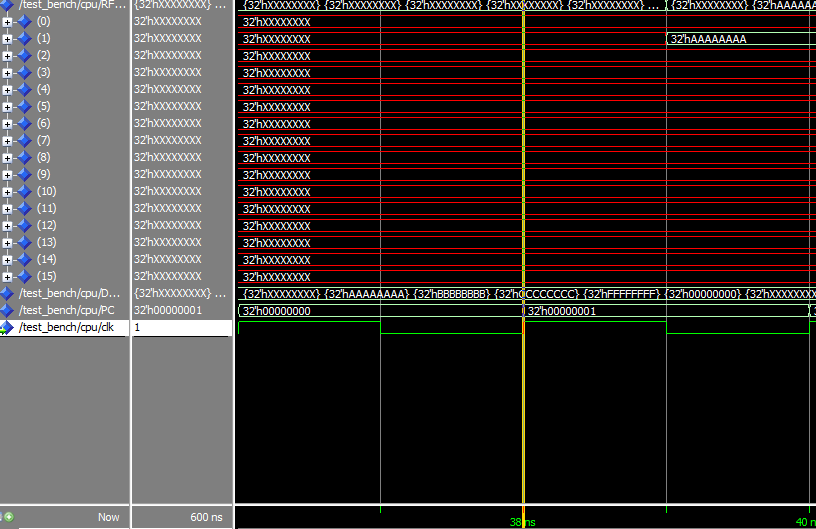
\includegraphics[width=\linewidth]{simulation/1-instr}
\caption{\texttt{lw \$s1, 1(\$zero)}}
\label{fig:1-instr}
\end{figure}

Figure \ref{fig:2-instr} shows the second instruction. The value of 0xAAAAAAAA in register \$s1 is successfully stored into the data memory at address 0x00000006.
\begin{figure}[H]
\centering
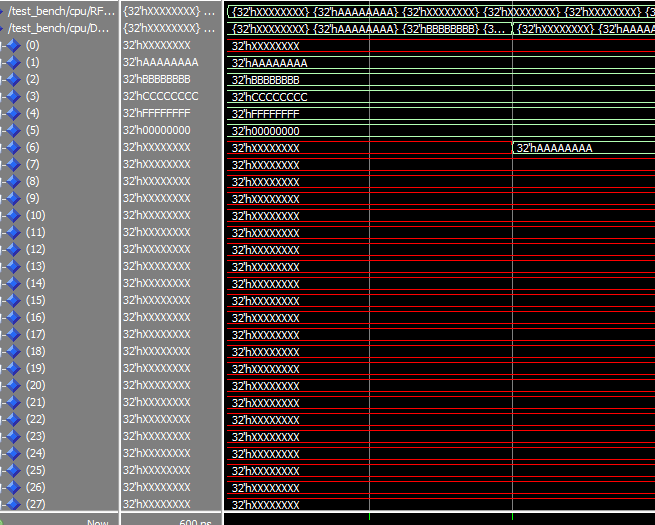
\includegraphics[width=\linewidth]{simulation/2-instr}
\caption{\texttt{sw \$s1, 6(\$zero)}}
\label{fig:2-instr}
\end{figure}

Figure \ref{fig:3-instr} shows the third instruction. The value of 0xBBBBBBBB at address 0x00000002 is successfully loaded into register \$s2.
\begin{figure}[H]
\centering
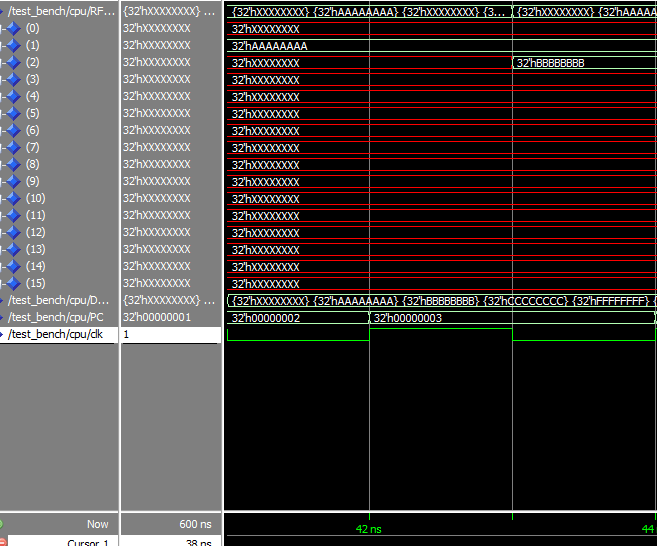
\includegraphics[width=\linewidth]{simulation/3-instr}
\caption{\texttt{lw \$s2, 2(\$zero)}}
\label{fig:3-instr}
\end{figure}

Figure \ref{fig:4-instr} shows the fourth instruction. The values of 0xAAAAAAAA and 0xBBBBBBBB are successfully added with the correct result of 0x66666665 being written into register \$s3.

\begin{figure}[H]
\centering
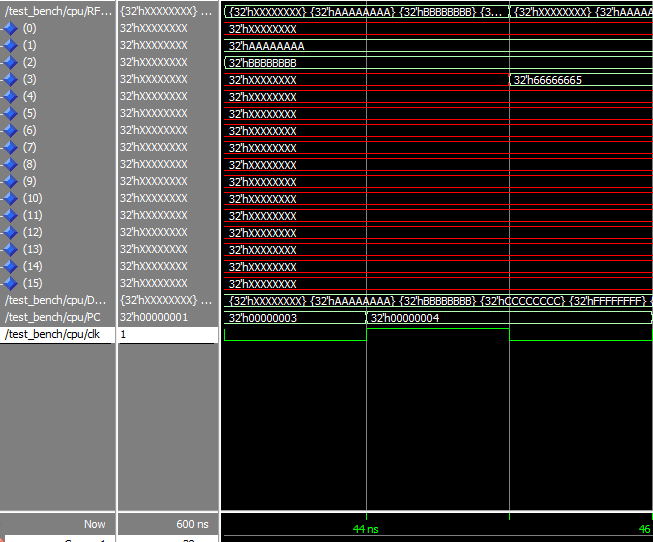
\includegraphics[width=\linewidth]{simulation/4-instr}
\caption{\texttt{add \$s3, \$s1, \$s2}}
\label{fig:4-instr}
\end{figure}

Figure \ref{fig:5-instr} shows the fifth instruction. The value of 0xAAAAAAAA in register \$s1 is subtracted from register \$s2. The result is 0x11111111 and is written back into register \$s4.
\begin{figure}[H]
\centering
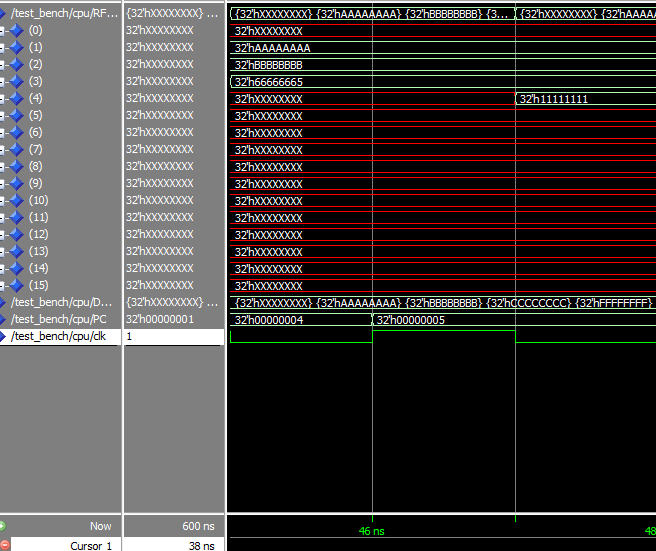
\includegraphics[width=\linewidth]{simulation/5-instr}
\caption{\texttt{sub \$s4, \$s2, \$s1}}
\label{fig:5-instr}
\end{figure}


Figure \ref{fig:6-instr} shows the sixth instruction. The value of 0xBBBBBBBB in register \$s2 is compared to 0xAAAAAAAA in register \$s1 for equivalence. Since they are not, the program counter increments to the next instruction.
\begin{figure}[H]
\centering
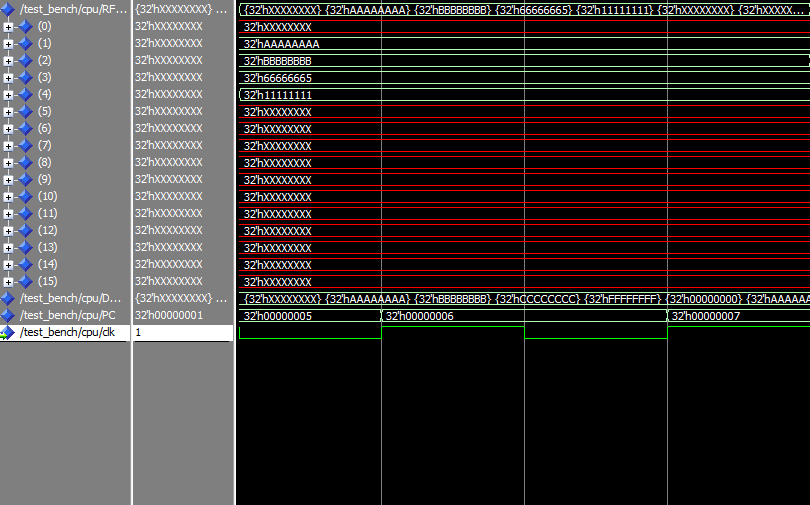
\includegraphics[width=\linewidth]{simulation/6-instr}
\caption{\texttt{beq \$s1, \$s2, 100}}
\label{fig:6-instr}
\end{figure}


Figure \ref{fig:7-instr} shows the seventh instruction. The value of 0xFFFFFFFF at address 0x00000004 is loaded into register \$s2 successfully.
\begin{figure}[H]
\centering
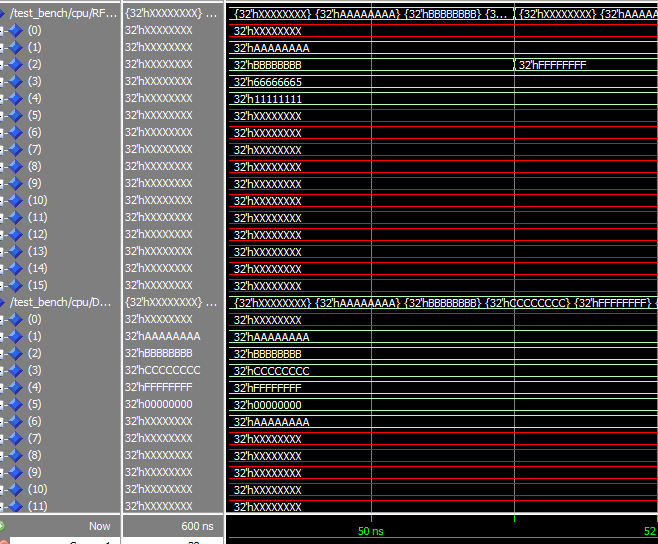
\includegraphics[width=\linewidth]{simulation/7-instr}
\caption{\texttt{lw \$s2, 4(\$zero)}}
\label{fig:7-instr}
\end{figure}

Figure \ref{fig:8-instr} shows the eighth instruction. The value of 0xFFFFFFFF in register \$s2 and 0xAAAAAAAA in register are nanded and the result of 0x55555555 is both accurate and stored in register \$s5.
\begin{figure}[H]
\centering
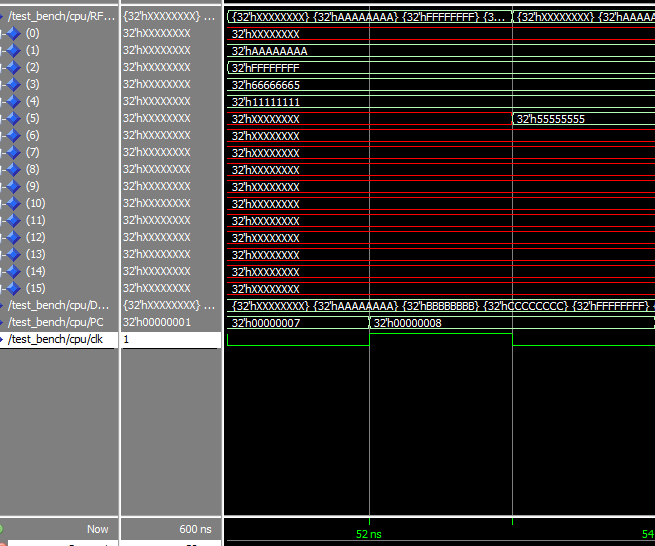
\includegraphics[width=\linewidth]{simulation/8-instr}
\caption{\texttt{nand \$s5, \$s1, \$s2}}
\label{fig:8-instr}
\end{figure}


Figure \ref{fig:9-instr} shows the ninth instruction. The immediate value of 0x000000FF is anded with the value of 0xFFFFFFFF in register \$s2. The correct result of 0x000000FF is calculated and written into register \$s6.
\begin{figure}[H]
\centering
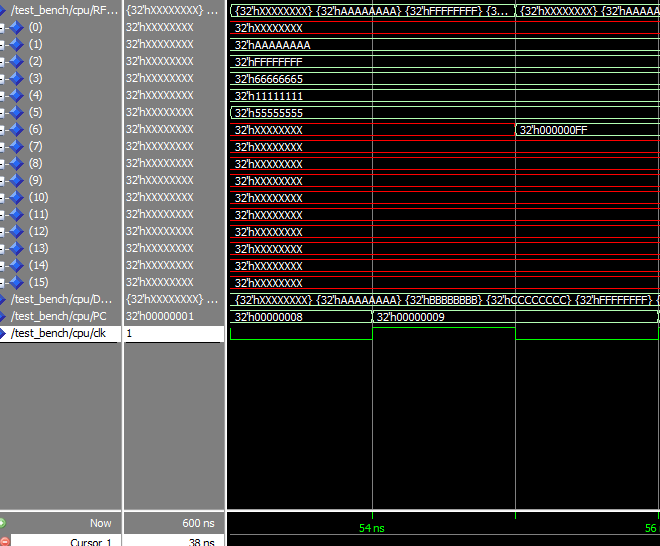
\includegraphics[width=\linewidth]{simulation/9-instr}
\caption{\texttt{andi \$s6, \$s2, 0x00FF}}
\label{fig:9-instr}
\end{figure}

Figure \ref{fig:10-instr} shows the tenth instruction. The immediate value of 0x000000FF is or'ed with the value of 0xAAAAAAAA in register \$s1. The correct result of 0xAAAAAAFF is written into register \$s7.
\begin{figure}[H]
\centering
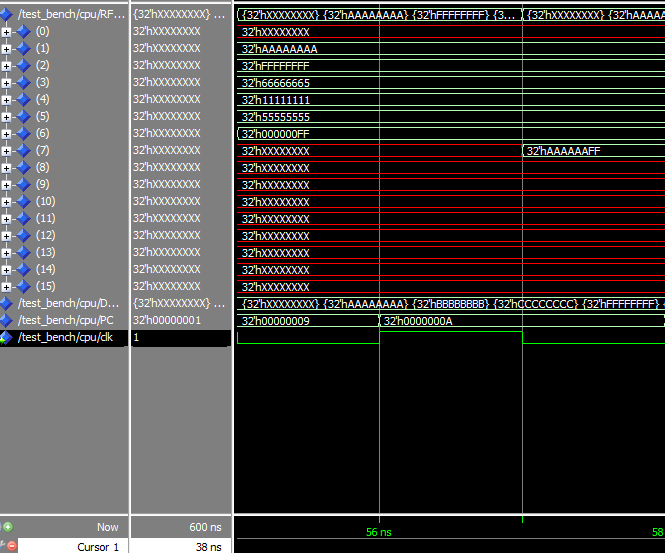
\includegraphics[width=\linewidth]{simulation/10-instr}
\caption{\texttt{ori \$s7, \$s1, 0x00FF}}
\label{fig:10-instr}
\end{figure}


Figure \ref{fig:11-instr} shows the eleventh instruction. The value of 0xFFFFFFFF in register \$s2 and 0xAAAAAAAA in register \$s1 are or'ed. The correct result of 0xFFFFFFFF is written into register \$s8.
\begin{figure}[H]
\centering
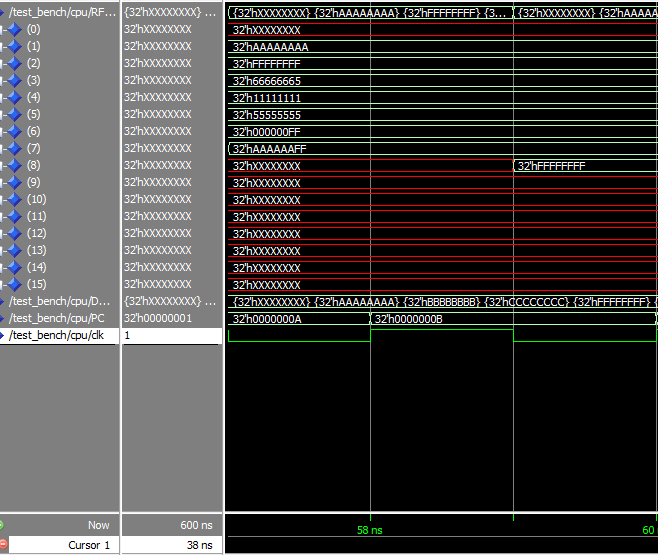
\includegraphics[width=\linewidth]{simulation/11-instr}
\caption{\texttt{or \$s8, \$s1, \$s2}}
\label{fig:11-instr}
\end{figure}


Figure \ref{fig:12-instr} shows the twelfth instruction. The value in register \$s1 is checked for equivalence with itself. Since it is equal, the program counter branches backwards successfully back to 0x00000001. Thus the test program infinitely loops. 
\begin{figure}[H]
\centering
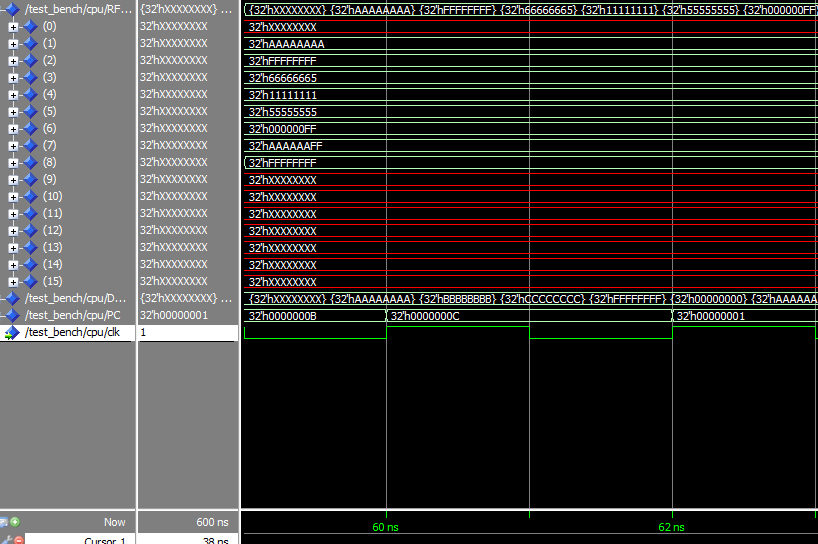
\includegraphics[width=\linewidth]{simulation/12-instr}
\caption{\texttt{beq \$s1, \$s1, -0x000B}}
\label{fig:12-instr}
\end{figure}


\section{Conclusion}
The design and implementation of a 32-bit CPU was a success. A set of 9 instructions were successfully implemented and verified with test bench code. All requested functionality was achieved. This 32-bit CPU can now be used in further projects and can be expanded upon to become a more efficient piece of hardware.
\newpage
\section*{Appendix}
\lstinputlisting[label=cpuCode, caption=CPU Code]{mips.vhd}
\lstinputlisting[label=tbCode, caption=Test Bench Code]{test_bench.vhd}\label{code:tbCode}

\end{document}
